\documentclass[12pt]{article}
\usepackage[utf8]{inputenc}
\usepackage{float}
\usepackage{amsmath}


\usepackage[hmargin=3cm,vmargin=6.0cm]{geometry}
%\topmargin=0cm
\topmargin=-2cm
\addtolength{\textheight}{6.5cm}
\addtolength{\textwidth}{2.0cm}
%\setlength{\leftmargin}{-5cm}
\setlength{\oddsidemargin}{0.0cm}
\setlength{\evensidemargin}{0.0cm}

%misc libraries goes here
\usepackage{comment}
\usepackage{booktabs}
\usepackage{enumitem}
%\usepackage{indentfirst}
\usepackage{amssymb}
\usepackage{tikz}


\begin{document}

\section*{Student Information } 
%Write your full name and id number between the colon and newline
%Put one empty space character after colon and before newline
Full Name : Deniz Koluaçık \\
Id Number : 2310274 \\

% Write your answers below the section tags
\section*{Answer 1}
\begin{enumerate}[label=\alph*)]
	\item
		We can treat the number of binary string of length $n$ that meet the given specification as a recurrence relation problem. We can create a binary string of length $n$ either by concatanating a ``0'' to a string of length $n-1$ or by concatanating a ``10'' to a string of length $n-2$. Thus, the formula for the linear recurrence relation is the following: \[a_n = a_{n-1} + a_{n-2}\]
		Where $a_1 = 1$ (0), and $a_2 = 2$ (10, 00). Clearly, what we get resembles the \textit{fibonacci sequence}. \[1,2,3,5,8,13,21,34,55\mathellipsis\] However since $``00\ldots0$'' is not considered a valid string, we will subtract 1 from our final result.  $a_9 = 55$ The answer is 54.
	\item
		Notice that the order of digits should be taken into consideration, and 1s and 0s are indistinguisable. We have 3 cases of bit strings in terms of the number of 1s and 0s they consist of.
		\begin{enumerate}[label=\roman*)]
			\item{} 8 1s and 2 0s:\\
				\[\dfrac{10!}{8!2!} = 45\]
			\item{} 9 1s and 1 0:\\
				\[\dfrac{10!}{9!1!} = 10\]
			\item{} 10 1s and no 0s:\\
				\[\dfrac{10!}{10!} = 1\]
		\end{enumerate}
		By \textbf{sum rule}, there are $45 + 10 + 1 = 56$ bit strings that meet the specifications.\\
	\item
		The number of onto functions from a set with $m$ elements to a set $n$ elements is \[n^m - \binom{n}{1}(n-1)^m + \binom{n}{2}(n-2)^m-\cdots+(-1)^{n-1}\binom{n}{n-1}1^m\]
		By \textit{Theorem 1 from section 8.6 (textbook)}. For $m=4$ and $n=3$, there are $81-48+3=36$ onto functions.
		\begin{comment}For a function $f$ from $A$, $(|A| = 4)$ to $B$, $(|B| = 3)$ to be onto, all elements of $B$ must be \textit{assigned to} a element of $A$. We can first guarantee \textit{being onto} property of $f$, then map the remaining elements of $A$ freely.
		\begin{enumerate}[label=\roman*)]
			\item We need to \textit{assign} three distinct elements of $A$ to three distinct elements of $B$\label{foo}.  %\[P(4,3) = 24\]
				\begin{equation}
					P(4,3) = 24
				\end{equation}
			\item We have one \textit{unassigned} element in $A$. Since our criterion is already met, we can \textit{assign} it freely. This can be done in three different ways since $s(B) = 3$\label{bar}.
		\end{enumerate}
		Finally, by \ref{foo} and \ref{bar}, there are $24 \times 3 = 72$ different onto functions by \textbf{product rule}.
		\end{comment}
	\item 
		\begin{comment}The order of the items is irrelevant as what being made is a collection. There are three different cases of such collections being made: 1D (Discrete Mathematics) and 3S (Signals and Systems), 2D and 2S, 3D and 1S. 
		\[\binom{5}{1}\binom{7}{3} + \binom{5}{2}\binom{7}{2} + \binom{5}{3}\binom{7}{1}=455\]
		\end{comment}
		Since books of the same courses are identical, and thus, indistinguisable, there are only three possible configurations: 
		\begin{enumerate}
			\item S,S,S,D
			\item S,S,D,D
			\item S,D,D,D
		\end{enumerate}
		The answer is 3.
\end{enumerate}


\section*{Answer 2}
\begin{enumerate}[label=\alph*)]
	
	\item{} 
		Let us start with comparing subsets of the sets $A=\{1,2,3\mathellipsis n\}$ and $B=\{1,2,3\mathellipsis (n-1)\}$ that contain no consecutive numbers, (for the rest of question we will ommit the phrase ``that do not contain consective numbers'' to avoid repetition. The reader should assume that all subsets that are mentioned follow the given criterion.). All subsets of $B$ are also subsets of $A$. Additionally $A$ has some subsets containing $n$.\\

Let $C=\{1,2,3\mathellipsis (n-2)\}$. All subsets of $B$ that are not also subsets of $C$ contain $(n-1)$. The number of those subsets that contain $(n-1)$ is $a_{n-1} - a_{n-2}$. The remaining subsets of $B$ do not contain $(n-1)$, and there are $a_{n-2}$ of them. Moving back to subsets of $A$, we can produce subsets that contain $n$ by ``adding'' $n$ to the subsets of $B$ that do not contain $(n-1)$ (there are $a_{n-2}$ of them). Hence, we can write $a_n$ in terms of $a_{n-1}$ and $a_{n-2}$: \[a_n=a_{n-1}+a_{n-2}\]
		Where $a_1 = 2$ ($\varnothing$, $\{1\}$), and $a_2 = 3$ ($\varnothing$, $\{1\}$, $\{2\}$).
	\item
		Let $G(x) = \sum_{k=0}^\infty a_kx^k$ be our generating function for $a_n$.
		\begin{align*}
			G(x) - xG(x) - x^2G(x) &= \sum_{k=0}^\infty a_kx^k-\sum_{k=1}^\infty a_{k-1}x^k - \sum_{k=2}^\infty a_{k-2}x^k\\
			&= a_0 + a_1x - a_0x + \sum_{k=2}^\infty(a_k - a_{k-1} -a_{k-2})x^k\\
			&= a_0 + a_1x - a_0x 
		\end{align*}
		Hence, \[G(x) = \frac{1+x}{1-x-x^2}\] We want to write this in the following form: $\frac{1}{1-ax}$.\\
		\begin{align*}
			G(x) &= \frac{1+x}{1-x-x^2}\\
			&= -\left(\frac{A}{x+\frac{1-\sqrt{5}}{2}} + \frac{B}{x+\frac{1+\sqrt{5}}{2}}\right)\\
		\end{align*}
		\center($\ A+B=1$ and $\frac{A+A\sqrt{5}}{2} + \frac{B-B\sqrt{5}}{2} = 1$, $A=\frac{1+\sqrt{5}}{2\sqrt{5}},B=\frac{-1+\sqrt{5}}{2\sqrt{5}}$)
		\begin{align*}
			G(x) &= \frac{1+x}{1-x-x^2}\\
			&= \frac{6+2\sqrt{5}}{4\sqrt{5}} \left(\frac{1}{1-\frac{\sqrt{5}+1}{2}x}\right)+\frac{6-2\sqrt{5}}{4\sqrt{5}}\left(\frac{1}{1-\frac{\sqrt{5}-1}{2}x}\right)\\
			&= \frac{6+2\sqrt{5}}{4\sqrt{5}} \sum_{k=0}^\infty {\left(\frac{\sqrt{5}+1}{2}\right)^kx^k}+ \frac{6-2\sqrt{5}}{4\sqrt{5}} \sum_{k=0}^\infty\left(\frac{\sqrt{5}-1}{2}\right)^kx^k\\
		\end{align*}
\end{enumerate}


\section*{Answer 3}
	$a_n$ is in the form $a_n = \alpha_1r_1^n + \alpha_2r_2^n + \alpha_3r_3^n$\\
The characteristic equation of the given recurrene relation is the following: \[r^3 - 4r^2 - r + 4=0\] whose roots are $r_1 = 1$, $r_2 = (-1)$, $r_3 = 4$. To find $\alpha_1$, $\alpha_2$, and $\alpha_3$, we need to solve the following system of equation for $\alpha_1$, $\alpha_2$, and $\alpha_3$.\\

\[
\begin{array}{ccccccc}
	\alpha_1 &+ &\alpha_2(-1)^0 &+& \alpha_34^0&=&4\\
	\alpha_1 &+ &\alpha_2(-1)^1 &+& \alpha_34^1&=&8\\
	\alpha_1 &+ &\alpha_2(-1)^2 &+& \alpha_34^2&=&34\\
\end{array}
\] \\

We see that $\alpha_1=1$, $\alpha_2=1$, and $\alpha_3=2$. Hence, \[a_n = 1 + (-1)^n + 2\times 4^n\]


\section*{Answer 4}
For $R$ to be a equivalence relation, it needs to be \textit{reflexive}, \textit{transitive}, and \textit{symmetric}.\\
	
\begin{enumerate}
	\item{}If $(x_1,y_1)R(x_1,y_1)$ then $R$ is reflexive. This is a trivial thing to do since $3x_1 - 2y_1 = 3x_1 - 2y_1$, obviously.
	\item{}For $R$ to be transitive, the following should be true: ``If $(x_1,y_1)R(x_2,y_2)$ and $(x_2,y_2)R(x_3,y_3)$, then $(x_1,y_1)R(x_3,y_3)$.''
		Let $3x_1 - 2y_1 = k$. If $(x_1,y_1)R(x_2,y_2)$, then $3x_2 - 2y_2 = k$, also. Similarly, if $(x_2,y_2)R(x_3,y_3)$, then $3x_3 - 3y_3=k$, also. Finally, since $3x_1-2y_1 = 3x_3 - 2y_3$, $(x_1,y_1)R(x_3,y_3)$. Thus, R is transitive.
	\item{}For $R$ to be symmetric the following should be true: ``If $(x_1,y_1)R(x_2,y_2)$, then $(x_2,y_2)R(x_1,y_1)$.'' Again, this is a trivial thing to do. $3x_1-2y_1 = 3x_2 - 2y_2$, then $3x_2 - 2y_2 = 3x_1 - 2y_1$, and $(x_2,y_2)R(x_1,y_1)$. Thus, $R$ is symmetric.\\

\end{enumerate}
		
			\begin{figure}[H]
				\centering
				
		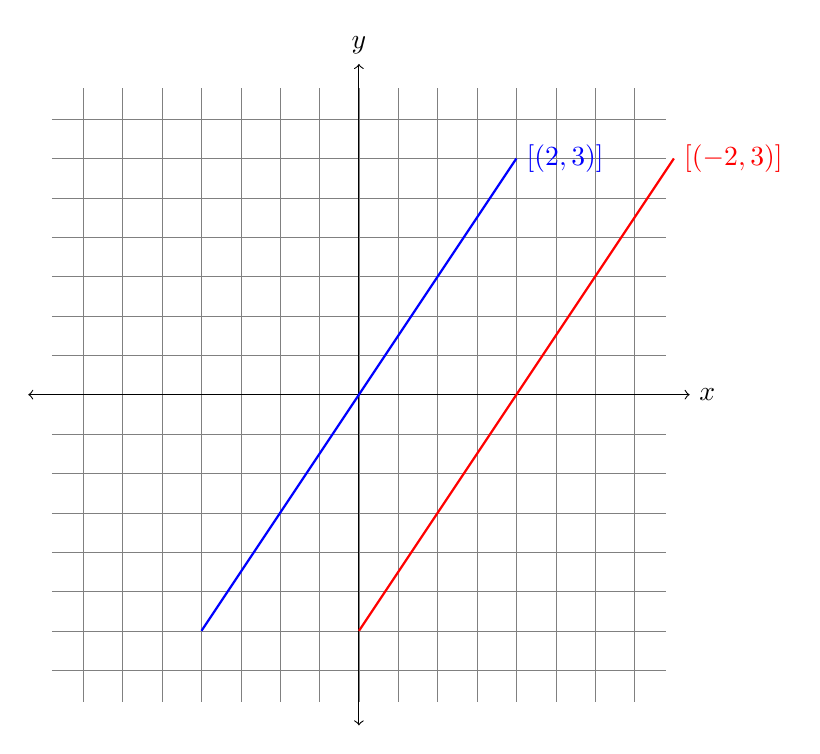
\begin{tikzpicture}[domain=0:6]
			\draw[step=0.5, very thin, color=gray] (-3.9,-3.9) grid (3.9,3.9);
			\draw[<->] (-4.2,0) -- (4.2,0) node[right] {$x$};
			\draw[<->] (0,-4.2) -- (0,4.2) node[above] {$y$};
			\draw[thick, color=red] (0,-3) -- (4,3) node[right] {$[(-2,3)]$};
			\draw[thick, color=blue] (-2,-3) -- (2,3) node[right] {$[(2,3)]$};
		\end{tikzpicture}
				\caption{The graphical representation of the given equivalence classes}
			\end{figure}
	




\end{document}
